\chapter{Conjuntos de instâncias de \textit{benchmark} dinâmicas}
\label{ch:instancias}
% TODO: o que são Instâncias de Benchmark Dinâmicas?
Como mencionado no Capítulo~\ref{ch:formulacao_problemas}, uma instância
simboliza uma determinada configuração dos parâmetros de um problema,
representado um cenário de aplicação do problema.
\textit{Benchmark}, por sua vez, simboliza o método de executar um conjunto de
testes padrões em um programa de computador com o objetivo de avaliar seu
desempenho \cite{fleming_how_1986}.

Para o nosso caso, os programas de computador seriam os algoritmos de
roteamento e os testes padrões consistem em achar as soluções para um conjunto 
de instâncias padrão, denominado conjunto de instâncias de \textit{benchmark}.
A avaliação de desempenho feita para esses casos é tanto no quesito de tempo
de computação como da qualidade da solução encontrada.
Portanto, para avanço de pesquisas que focam no desenvolvimento de algoritmos,
é interessante que existam conjuntos de instâncias de
\textit{benchmark} de referência, para que estes algoritmos possam ser
comparados de forma direta.

Entretanto, \textcite{pillac_review_2013} argumenta que não existe nenhum
conjunto de instâncias de \textit{benchmark} de referência para os problemas 
de roteamento dinâmico.
A prática mais comum é a adaptação e utilização de instâncias de 
\textit{benchmark} estáticas através de métodos que distribuem os instantes de 
chegada dos pedidos ($\arrivalTime_\request$) ao longo do horizonte de
planejamento.
Contudo, \textcite{maciejewski_towards_2017} comenta que essa abordagem é 
problemática.
Eles mencionam, como exemplo, que é impossível em uma instância estática fazer 
o sistema reagir ao controle, como no caso de um cancelamento de pedido quando 
a coleta leva muito tempo. 
Também comentam que mesmo simples sequências de eventos pré planejados podem
gerar inconsistências no sistema, como por exemplo o cancelamento de um pedido
que já foi coletado.
Portanto, a falta de instâncias de \textit{benchmark} devidamente apropriadas e
que sejam conhecidas por sua boa qualidade acarreta em um uso de diferentes 
instâncias em diferentes artigos, dificultando a comparação de desempenho dos 
algoritmos.

Esta seção tem como objetivo apresentar seis conjuntos de instâncias de 
\textit{benchmark} dinâmicas DDARP ou DPDPTW cujos os dados estão disponíveis 
para acesso na internet \cite{pankratz_benchmark_2009} e que
serão analisados no Capítulo~\ref{ch:analise}.
Quatro desses conjuntos de instâncias dinâmicas são derivados de conjuntos 
estáticos: 
\textcite{berbeglia_hybrid_tabu_2012},
\textcite{pureza_laporte_waiting_2008}, 
\textcite{pankratz_dynamic_2005}
e \textcite{fabri_dynamic_2006}
aplicam, cada um, um método diferente para transformar as
instâncias estáticas em dinâmicas.
O quinto conjunto foi criado artificialmente por 
\textcite{gendreau_neighborhood_2006} de maneira a replicar o comportamento de 
um centro urbano, com horários de pico e uma demanda concentrada no centro da 
cidade.
O sexto conjunto é baseado em dados reais, coletados em duas companhias 
de correio de médio e grande porte, que operam em Vancouver, Canadá 
\cite{mitrovic-minic_waiting_2004}.
Os métodos de dinamização ou as formas de alocação temporal dos pedidos de cada
um dos conjuntos serão apresentados nesta seção.

Destaca-se que todos os dados dos conjuntos de instâncias de \textit{benchmark}
que serão caracterizados e analisados estão disponíveis para consulta e
utilização, assim como todos os códigos usados para a análise destas
instâncias \cite{eccel_problemas_2019}.

A Tabela~\ref{tab:instancias} mostra as características gerais das instâncias
estudadas.

\begin{table}[]
\newcommand{\firstColumnWidth}{1.52cm}
\newcommand{\columnWidth}{2.25cm}
\newcommand{\numberOfRows}{2}
\footnotesize
\caption{Características estáticas dos conjuntos de instâncias de 
         \textit{benchmark}}
\label{tab:instancias}
\begin{tabular}{llllll}
\toprule
\multirow{4}{\columnWidth}{} & 
  \multirow{\numberOfRows}{\columnWidth}{\textcite{ropke_models_2007}} & 
  \multirow{\numberOfRows}{\columnWidth}{\textcite{cordeau_tabu_2003}} & 
  \multirow{\numberOfRows}{\columnWidth}{\textcite{li_metaheuristic_2003}} & 
  \multirow{\numberOfRows}{\columnWidth}{
    \textcite{gendreau_neighborhood_2006}} & 
  \multirow{\numberOfRows}{\columnWidth}{
    \textcite{mitrovic-minic_waiting_2004}}
\\ & & & & & \\ & & & & & \\ & & & & & \\   
\midrule
\multirow{\numberOfRows}{\firstColumnWidth}{N. de instâncias} & 
  \multirow{\numberOfRows}{\columnWidth}{42} & 
  \multirow{\numberOfRows}{\columnWidth}{20} & 
  \multirow{\numberOfRows}{\columnWidth}{354} & 
  \multirow{\numberOfRows}{\columnWidth}{15} & 
  \multirow{\numberOfRows}{\columnWidth}{220}
\\ & & & & & \\
\multirow{\numberOfRows}{\firstColumnWidth}{$\planingHorizon$ (min)} & 
  \multirow{\numberOfRows}{\columnWidth}{1440} & 
  \multirow{\numberOfRows}{\columnWidth}{1440} & 
  \multirow{\numberOfRows}{\columnWidth}{[1236, 3693]} & 
  \multirow{\numberOfRows}{\columnWidth}{240 ou 450} & 
  \multirow{\numberOfRows}{\columnWidth}{600}
\\ & & & & & \\
  \multirow{\numberOfRows}{\firstColumnWidth}{Geometria ($\text{km}^2$)} & 
  \multirow{\numberOfRows}{\columnWidth}{10 $\times$ 10} & 
  \multirow{\numberOfRows}{\columnWidth}{10 $\times$ 10} & 
  \multirow{\numberOfRows}{\columnWidth}{100 $\times$ 100} & 
  \multirow{\numberOfRows}{\columnWidth}{5 $\times$ 5} & 
  \multirow{\numberOfRows}{\columnWidth}{60 $\times$ 60}
\\ & & & & & \\
\multirow{\numberOfRows}{\firstColumnWidth}{$\numberOfRequests$} & 
  \multirow{\numberOfRows}{\columnWidth}{[16, 96]} & 
  \multirow{\numberOfRows}{\columnWidth}{[24, 144]} & 
  \multirow{\numberOfRows}{\columnWidth}{[50, 500]} & 
  \multirow{\numberOfRows}{\columnWidth}{[84, 217]} & 
  \multirow{\numberOfRows}{\columnWidth}{[100, 1000]}
\\ & & & & & \\
\multirow{\numberOfRows}{\firstColumnWidth}{$|\vehiclesSet|$}  &
  \multirow{\numberOfRows}{\columnWidth}{[2, 8]} & 
  \multirow{\numberOfRows}{\columnWidth}{[3, 13]} & 
  \multirow{\numberOfRows}{\columnWidth}{[25, 500]} & 
  \multirow{\numberOfRows}{\columnWidth}{10 ou 20} & 
  \multirow{\numberOfRows}{\columnWidth}{[20, 80]}
\\ & & & & & \\
\multirow{\numberOfRows}{\firstColumnWidth}{$\vehicleCapacity$}  &  
  \multirow{\numberOfRows}{\columnWidth}{3 ou 6 } & 
  \multirow{\numberOfRows}{\columnWidth}{6} & 
  \multirow{\numberOfRows}{\columnWidth}{[200, 1000]} & 
  \multirow{\numberOfRows}{\columnWidth}{$\infty$} & 
  \multirow{\numberOfRows}{\columnWidth}{$\infty$}
\\ & & & & & \\
  \multirow{\numberOfRows}{\firstColumnWidth}{$\nodeLoad{\request}$} &
  \multirow{\numberOfRows}{\columnWidth}{[1, 6]} & 
  \multirow{\numberOfRows}{\columnWidth}{1} & 
  \multirow{\numberOfRows}{\columnWidth}{[3, 36]} & 
  \multirow{\numberOfRows}{\columnWidth}{1} & 
  \multirow{\numberOfRows}{\columnWidth}{1}
\\ & & & & & \\
\multirow{\numberOfRows}{\firstColumnWidth}{$\serviceTime_\request$ (min)} & 
  \multirow{\numberOfRows}{\columnWidth}{[1, 6]} & 
  \multirow{\numberOfRows}{\columnWidth}{10} & 
  \multirow{\numberOfRows}{\columnWidth}{90} & 
  \multirow{\numberOfRows}{\columnWidth}{5} & 
  \multirow{\numberOfRows}{\columnWidth}{0}
\\ & & & & & \\
\multirow{\numberOfRows}{\firstColumnWidth}{$\vehicleMaxRouteTime$  (min)}  &
  \multirow{\numberOfRows}{\columnWidth}{[480, 720]} & 
  \multirow{\numberOfRows}{\columnWidth}{480} & 
  \multirow{\numberOfRows}{\columnWidth}{[1236, 3693]} & 
  \multirow{\numberOfRows}{\columnWidth}{240 ou 450} & 
  \multirow{\numberOfRows}{\columnWidth}{600}
\\ & & & & & \\
\multirow{\numberOfRows}{\firstColumnWidth}{$\maxRideTime_\request$ (min)}  &
  \multirow{\numberOfRows}{\columnWidth}{30 ou 45} & 
  \multirow{\numberOfRows}{\columnWidth}{90} & 
  \multirow{\numberOfRows}{\columnWidth}{[1236, 3693]} & 
  \multirow{\numberOfRows}{\columnWidth}{240 ou 450} & 
  \multirow{\numberOfRows}{\columnWidth}{600}
\\ & & & & & \\
\bottomrule
\end{tabular}
\end{table}





\section{Conjunto de instâncias DDARP propostas por 
         Berbeglia, Cordeau e Laporte (2012)}
\label{sec:instances_berbeglia}

\textcite{berbeglia_hybrid_tabu_2012} usam dois diferentes conjuntos de 
instâncias para seus experimentos, cada um deles sendo derivado de conjuntos 
de instâncias estáticas diferentes.
O primeiro conjunto tem como base as instâncias estáticas propostas por 
\textcite{ropke_models_2007}.
Já no segundo são usadas as instâncias estáticas apresentadas por
\textcite{cordeau_tabu_2003}.
Destaca-se que \textcite{berbeglia_hybrid_tabu_2012} usaram apenas as 
instâncias estáticas com no mínimo 40 pedidos.
% TODO: Qual a relevância disso? Em que escala de tempo?
O restante dessa seção apresenta em detalhes cada um desses conjuntos, assim
como o método usado para dinamizá-los.

\subsection{Primeiro conjunto}\label{sec:instances_berbeglia_1}
\textcite{berbeglia_hybrid_tabu_2012} usam como base as instâncias estáticas 
propostas por \textcite{ropke_models_2007} que, por sua vez, utilizaram o 
método proposto por \textcite{savelsbergh_drive:_1998} para geração de 
instâncias estáticas.
Destaca-se que essas mesmas instâncias estáticas foram usadas também por
\textcite{cordeau_branch-and-cut_2006}.

Neste conjunto de instâncias os pedidos estão contidos em um plano Euclidiano
delimitado por uma área de $20 \times 20 \text{ km}^2$, sendo que a 
distribuição espacial dos nós de coleta e de entrega é gerada através do 
sorteio de uma variável com distribuição aleatória uniforme.
Os pedidos são divididos em duas categorias, pedidos de coleta e pedidos de
entrega, sendo que o primeiro só possui uma janela de tempo definida na coleta 
e o segundo apenas janela de tempo de entrega.
O horizonte de planejamento é de 12 horas e as janelas de tempo são de 15
minutos.

Dentro deste conjunto de instâncias existem os subconjuntos ``a'' e ``b'',
que diferenciam entre si pelos valores de capacidade dos veículos 
($\capacity_\request$), do tempo máximo de viagem de um pedido 
($\maxRideTime_\request$), do carregamento dos pedidos 
($\load_\request$) e do tempo de serviço ($\serviceTime_i$).
No subconjunto ``a'' esses valores são: $\vehicleCapacity = 3, \forall
\vehicle \in \vehiclesSet$ e $\load_\request = 1, \serviceTime_\request = 1\ 
\text{min}, \maxRideTime_\request = 30\ \text{min}, \forall \request \in
\requests$.
No subconjunto ``b'' esses valores são: $\vehicleCapacity = 6, \forall
\vehicle \in \vehiclesSet$ e $\load_\request = \uniformDistribution{1}
{\vehicleCapacity}, \serviceTime_\request = \load_\request, 
\maxRideTime_\request = 45\ \text{min}, \forall \request \in \requests$.

Esses subconjuntos foram criados para representar o caso em que carros são
usados para o transporte dos usuários (``a'') e o caso em que mini-ônibus 
seriam usados para o mesmo fim (``b'').

Por fim, a Tabela~\ref{tab:ropke_models_2007_DARP_instances_caracteristics}
apresenta algumas das características das instâncias estáticas de ambos os 
subconjuntos propostos por \textcite{ropke_models_2007}, isto é, antes da
dinamização.

% TODO: apresentar as instâncias com <40 pedidos?

\begin{table}[h]
\footnotesize
  \centering
  \caption{Características das instâncias DARP de 
           \textcite{ropke_models_2007}}
  \newcommand{\qib}{$\uniformDistribution{1}{\vehicleCapacity}$}
  \label{tab:ropke_models_2007_DARP_instances_caracteristics}
  \begin{tabular}{lrrrrrr|lrrrrrr}
    \toprule
    \multicolumn{7}{c|}{Subconjunto ``a''} &
    \multicolumn{7}{c}{Subconjunto ``b''} \\
    ID & $\vehiclesSetSize$ & $\numberOfRequests$ & $\maxRouteTime_\request$ & 
    $\load_\request$ & $\capacity_\vehicle$ & $\maxRideTime_\request$ & 
    ID & $\vehiclesSetSize$ & $\numberOfRequests$ & $\maxRouteTime_\request$ & 
    $\load_\request$ & $\capacity_\vehicle$ & $\maxRideTime_\request$\\
    \midrule
    a2-16 & 2 & 16 & 480 & 1 & 3 & 30 & b2-16 & 2 & 16 & 480 & \qib & 6 & 45\\
    a2-20 & 2 & 20 & 600 & 1 & 3 & 30 & b2-20 & 2 & 20 & 600 & \qib & 6 & 45\\
    a2-24 & 2 & 24 & 720 & 1 & 3 & 30 & b2-24 & 2 & 24 & 720 & \qib & 6 & 45\\
    a3-24 & 3 & 24 & 480 & 1 & 3 & 30 & b3-24 & 3 & 24 & 480 & \qib & 6 & 45\\
    a3-30 & 3 & 30 & 600 & 1 & 3 & 30 & b3-30 & 3 & 30 & 600 & \qib & 6 & 45\\
    a3-36 & 3 & 36 & 720 & 1 & 3 & 30 & b3-36 & 3 & 36 & 720 & \qib & 6 & 45\\
    a4-32 & 4 & 32 & 480 & 1 & 3 & 30 & b4-32 & 4 & 32 & 480 & \qib & 6 & 45\\
    a4-40 & 4 & 40 & 600 & 1 & 3 & 30 & b4-40 & 4 & 40 & 600 & \qib & 6 & 45\\
    a4-48 & 4 & 48 & 720 & 1 & 3 & 30 & b4-48 & 4 & 48 & 720 & \qib & 6 & 45\\
    a5-40 & 5 & 40 & 480 & 1 & 3 & 30 & b5-40 & 5 & 40 & 480 & \qib & 6 & 45\\
    a5-50 & 5 & 50 & 600 & 1 & 3 & 30 & b5-50 & 5 & 50 & 600 & \qib & 6 & 45\\
    a5-60 & 5 & 60 & 720 & 1 & 3 & 30 & b5-60 & 5 & 60 & 720 & \qib & 6 & 45\\
    a6-48 & 6 & 48 & 480 & 1 & 3 & 30 & b6-48 & 6 & 48 & 480 & \qib & 6 & 45\\
    a6-60 & 6 & 60 & 600 & 1 & 3 & 30 & b6-60 & 6 & 60 & 600 & \qib & 6 & 45\\
    a6-72 & 6 & 72 & 720 & 1 & 3 & 30 & b6-72 & 6 & 72 & 720 & \qib & 6 & 45\\
    a7-56 & 7 & 56 & 480 & 1 & 3 & 30 & b7-56 & 7 & 56 & 480 & \qib & 6 & 45\\
    a7-70 & 7 & 70 & 600 & 1 & 3 & 30 & b7-70 & 7 & 70 & 600 & \qib & 6 & 45\\
    a7-84 & 7 & 84 & 720 & 1 & 3 & 30 & b7-84 & 7 & 84 & 720 & \qib & 6 & 45\\
    a8-64 & 8 & 64 & 480 & 1 & 3 & 30 & b8-64 & 8 & 64 & 480 & \qib & 6 & 45\\
    a8-80 & 8 & 80 & 600 & 1 & 3 & 30 & b8-80 & 8 & 80 & 600 & \qib & 6 & 45\\
    a8-96 & 8 & 96 & 720 & 1 & 3 & 30 & b8-96 & 8 & 96 & 720 & \qib & 6 & 45\\
    \bottomrule
  \end{tabular}
\end{table}

% TODO: Rodrigo: O que se pode dizer qualitativamente a respeito dessas
% instâncias?

\subsection{Segundo conjunto}\label{sec:instances_berbeglia_2}

Conjunto com vinte instâncias estáticas criado por \textcite{cordeau_tabu_2003}
a partir de dados reais obtidos em campo. 
As informações relativas ao tamanho das janelas de tempo, 
capacidade dos veículos, tempo máximo de rota e tempo máximo de
viagem foram fornecidas pela \textit{Montreal Transit Commission}.

As instâncias foram geradas aleatoriamente e contêm entre 24 e 144 pedidos. 
Assim como no conjunto de instâncias apresentado na
Seção~\ref{sec:instances_berbeglia_1}, os pedidos estão localizados em uma 
área de $20 \times 20 \text{km}^2$ sendo que metade são pedidos que possuem
apenas janelas de tempo de coleta e a outra metade apenas na entrega.

Entretanto, diferente do conjunto apresentado na 
Seção~\ref{sec:instances_berbeglia_1}, os pedidos não são alocados usando uma
distribuição uniforme, mas sim determinados pelo procedimento descrito em
\textcite{cordeau_tabu_1997}, que cria agrupamentos de nós ao redor de um
certo número de pontos sementes.
A localização do depósito é determinada pela média dos pontos sementes.

O conjunto de instâncias estáticas de \textcite{cordeau_tabu_2003} apresenta
dois subconjuntos, cuja diferença é dada na forma de geração das janelas de
tempo.
No subconjunto ``a'', janelas de tempo curtas são geradas usando uma
distribuição uniforme dentro do intervalo $[60, 480]$ para a determinar o 
limite inferior ($\earliestTimeWindow_\originIndex$) da janela de tempo de 
coleta:
%
\begin{equation}
  \earliestTimeWindow_\originIndex = \uniformDistribution{60}{480}.
  \label{eq:instances_berbeglia_2_earliestTimeWindow}
\end{equation}

\noindent Logo em seguida, determina-se o limite superior da janela de coleta 
por:
%
\begin{equation}
  \latestTimeWindow_{\destinationIndex}  = \uniformDistribution
  {\earliestTimeWindow_\originIndex + 15}
  {\earliestTimeWindow_\originIndex + 45}.
  \label{eq:instances_berbeglia_2_a_latestTimeWindow}
\end{equation}

\noindent No subconjunto ``b'', janelas de tempo longas são criadas através da
determinação dos limites inferiores e superiores da janela de tempo de coleta.
Para isso as Equações~\ref{eq:instances_berbeglia_2_earliestTimeWindow}~e
\ref{eq:instances_berbeglia_2_b_latestTimeWindow}
%
\begin{equation}
  \latestTimeWindow_{\destinationIndex} = 
  \uniformDistribution
  {\earliestTimeWindow_\originIndex + 30}
  {\earliestTimeWindow_\originIndex + 90}.
  \label{eq:instances_berbeglia_2_b_latestTimeWindow}
\end{equation}

\noindent Para todas as instâncias, o tempo de rota máxima é 480 minutos, enquanto a
capacidade de cada veículo é igual a 6 e o carregamento de todos os pedidos
igual a 1.
Por último, o tempo máximo de viagem é igual a 90 minutos e o horizonte de
planejamento é de 1440 minutos (24 horas x 60 minutos).

A Tabela~\ref{tab:cordeau_tabu_2003_DARP_intances_characteristics} apresenta as
características gerais de cada uma das instâncias apresentadas por
\textcite{cordeau_tabu_2003}.

\begin{table}[h]
\footnotesize
  \centering
  \caption{Características das instâncias DARP de 
           \textcite{cordeau_tabu_2003}}
  \label{tab:cordeau_tabu_2003_DARP_intances_characteristics}
  \begin{tabular}{lrr|lrr}
    \toprule  
    \multicolumn{3}{c|}{Subconjunto ``a''} & 
    \multicolumn{3}{c}{Subconjunto ``b''} \\
    ID & $\numberOfRequests$ & $\vehiclesSetSize$ & 
    ID & $\numberOfRequests$ & $|\vehiclesSet|$\\
    \midrule
      R1a  &  24 &  3 & R1b  &  24 &  3\\
      R2a  &  48 &  5 & R2b  &  48 &  5\\
      R3a  &  72 &  7 & R3b  &  72 &  7\\
      R4a  &  96 &  9 & R4b  &  96 &  9\\
      R5a  & 120 & 11 & R5b  & 120 & 11\\
      R6a  & 144 & 13 & R6b  & 144 & 13\\
      R7a  &  36 &  4 & R7b  &  36 &  4\\
      R8a  &  72 &  6 & R8b  &  72 &  6\\
      R9a  & 108 &  8 & R9b  & 108 &  8\\
      R10a & 144 & 10 & R10b & 144 & 10\\
    \bottomrule
  \end{tabular}
\end{table}

\subsection{Método de dinamização de instâncias estáticas}

Esta seção se dedica a explicar o método usado por
\textcite{berbeglia_hybrid_tabu_2012} para transformar as instâncias
estáticas apresentadas nas
Seções~\ref{sec:instances_berbeglia_1}~e~\ref{sec:instances_berbeglia_2} em
instâncias dinâmicas.

% TODO: Ser menos direto nas definições
Define-se um par de parâmetros $(\staticPercentage,\maneuverTime)$;
$\staticPercentage \in [0, 1]$ define a porcentagem de pedidos conhecidos no 
início do horizonte de tempo.
Se $\staticPercentage = 0$ o problema é totalmente dinâmico, 
se $\staticPercentage = 1$ o problema é totalmente estático e todos os pedidos
são conhecidos previamente.  
$\maneuverTime$ representa um intervalo de tempo de reação do sistema aos
pedidos dinâmicos. Ou seja, intervalo entre a chegada do pedido e a sua coleta 
sempre será maior que $\beta$.

Dado um pedido $\request$, o valor $\requestLatestArrivalTime$  consiste em um
limite superior para o instante que o pedido deve ser conhecido para que seja
possível servi-lo. Assim:
%
\begin{equation}
    \requestLatestArrivalTime = 
    \min\{\latestTimeWindow_{\originIndex},
    \ \latestTimeWindow_{\destinationIndex}  
    - \arcTravelTime{\originIndex}{\destinationIndex} 
    - \serviceTime_{\request}\}.
    \label{eq:berbeglia_hybrid_2012_requestLatestArrivalTime}
\end{equation}

\noindent Portanto, o instante de chegada do pedido pode ser definido como:
%
\begin{equation}
    \requestArrivalTime = \requestLatestArrivalTime - \maneuverTime.
    \label{eq:berbeglia_hybrid_2012_requestArrivalTime}
\end{equation}

% TODO: Rodrigo: Qualitativamente, o que isso significa?

\noindent \textcite{berbeglia_hybrid_tabu_2012} utilizam os parâmetros 
$\staticPercentage = 0{,}25$ e $\maneuverTime = 60$ para a dinamização das 
instâncias apresentadas por \textcite{ropke_models_2007}.
Já o conjunto de instâncias pertencentes à \textcite{cordeau_tabu_2003}, foi 
transformado em um conjunto de instâncias dinâmicas usando os parâmetros 
$\staticPercentage = 0{,}25$ e $\maneuverTime =\uniformDistribution{60}{240}$.

Destaca-se que o presente trabalho usa o mesmo método de dinamização, porém usa 
$\alpha = 0$, já que o interesse é obter casos totalmente dinâmicos.

%TODO Rodrigo: Porque existe esse interesse?



\section{Conjunto de instâncias DPDPTW propostas por 
Pureza e Laporte (2008)}
\label{sec:pureza_instances}
% TODO Rodrigo: Qual a relevância do artigo li_metaheuristics_2003?

As instâncias DPDPTW propostas por \textcite{pureza_laporte_waiting_2008} 
foram geradas através da dinamização das instâncias estáticas com 100, 200 e 
400 nós (50, 100 e 200 pedidos) propostas por 
\textcite{li_metaheuristic_2003} que por sua vez, tiveram como base as 
instâncias VRPTW de 100 pedidos, criadas por 
\textcite{solomon_algorithms_1987}.

Seguindo a classificação de \textcite{solomon_algorithms_1987},  
\textcite{li_metaheuristic_2003} organizaram as instâncias em seis classes, 
identificadas por LC1, LC2, LR1, LR2, LRC1 e LRC2, indicando as respectivas 
distribuições espaciais dos nós e o tamanho dos horizontes de planejamento.
Nos conjuntos LC1 e LC2 os nós são agrupados, enquanto LR1 e LR2 possuem nós 
aleatoriamente distribuídos.
Os nós presentes nas instâncias LCR1 e LCR2 são parcialmente agrupados e 
parcialmente distribuídos aleatoriamente.
As instancias LC1, LR1 e LRC1 possuem um horizonte de planejamento curto, 
enquanto LC2, LR2 e LRC1 possuem um horizonte longo.

% TODO Rodrigo: O que o parágrafo anterior quer dizer?

A Tabela~\ref{tab:li_metaheuristics_2003_PDPTW_instances_characteristics}
apresenta algumas características das instâncias estáticas de
\textcite{li_metaheuristic_2003}.

\begin{footnotesize}
\begin{center}
\begin{longtable}{lrrr|lrrr|lrrr}
%    \caption{Características das instâncias PDPTW de 
%             \textcite{li_metaheuristic_2003}}
%    \label{tab:li_metaheuristics_2003_PDPTW_instances_characteristics}
        \hline
        ID & $\planingHorizon$ & $\numberOfRequests$ & $\vehicleCapacity$ & 
        ID & $\planingHorizon$ & $\numberOfRequests$ & $\vehicleCapacity$ & 
        ID & $\planingHorizon$ & $\numberOfRequests$ & $\vehicleCapacity$ \\ 
        \hline
        LC101      & 1236 &  53 & 200 & LR101      &  230 &  53 &  200 & LRC101      &  240 &  53 &  200\\
        LC102      & 1236 &  53 & 200 & LR102      &  230 &  55 &  200 & LRC102      &  240 &  53 &  200\\
        LC103      & 1236 &  52 & 200 & LR103      &  230 &  52 &  200 & LRC103      &  240 &  53 &  200\\
        LC104      & 1236 &  53 & 200 & LR104      &  230 &  52 &  200 & LRC104      &  240 &  54 &  200\\
        LC105      & 1236 &  53 & 200 & LR105      &  230 &  53 &  200 & LRC105      &  240 &  54 &  200\\
        LC106      & 1236 &  53 & 200 & LR106      &  230 &  52 &  200 & LRC106      &  240 &  53 &  200\\
        LC107      & 1236 &  53 & 200 & LR107      &  230 &  52 &  200 & LRC107      &  240 &  53 &  200\\
        LC108      & 1236 &  53 & 200 & LR108      &  230 &  50 &  200 & LRC108      &  240 &  52 &  200\\
        LC109      & 1236 &  53 & 200 & LR109      &  230 &  53 &  200 &             &      &     &     \\ 
                   &      &     &     & LR110      &  230 &  52 &  200 &             &      &     &     \\ 
                   &      &     &     & LR111      &  230 &  54 &  200 &             &      &     &     \\
                   &      &     &     & LR112      &  230 &  53 &  200 &             &      &     &     \\
                   &      &     &     &            &      &     &      &             &      &     &     \\
        LC201      & 3390 &  51 & 700 & LR201      & 1000 &  51 & 1000 & LRC201      & 1000 &  51 & 1000\\
        LC202      & 3390 &  51 & 700 & LR202      & 1000 &  50 & 1000 & LRC202      & 1000 &  51 & 1000\\
        LC203      & 3390 &  51 & 700 & LR203      & 1000 &  51 & 1000 & LRC203      & 1000 &  51 & 1000\\
        LC204      & 3390 &  51 & 700 & LR204      & 1000 &  50 & 1000 & LRC204      & 1000 &  51 & 1000\\
        LC205      & 3390 &  51 & 700 & LR205      & 1000 &  51 & 1000 & LRC205      & 1000 &  51 & 1000\\
        LC206      & 3390 &  51 & 700 & LR206      & 1000 &  50 & 1000 & LRC206      & 1000 &  51 & 1000\\
        LC207      & 3390 &  51 & 700 & LR207      & 1000 &  51 & 1000 & LRC207      & 1000 &  51 & 1000\\
        LC208      & 3390 &  51 & 700 & LR208      & 1000 &  50 & 1000 & LRC208      & 1000 &  51 & 1000\\
                   &      &     &     & LR209      & 1000 &  51 & 1000 &             &      &     &     \\
                   &      &     &     & LR210      & 1000 &  51 & 1000 &             &      &     &     \\
                   &      &     &     & LR211      & 1000 &  50 & 1000 &             &      &     &     \\
        \hline
        LC1\_2\_1  & 1351 & 106 & 200 & LR1\_2\_1  &  634 & 105 &  200 & LRC1\_2\_1  &  634 & 106 &  200\\
        LC1\_2\_2  & 1351 & 105 & 200 & LR1\_2\_2  &  634 & 105 &  200 & LRC1\_2\_2  &  634 & 103 &  200\\
        LC1\_2\_3  & 1351 & 103 & 200 & LR1\_2\_3  &  634 & 104 &  200 & LRC1\_2\_3  &  634 & 105 &  200\\
        LC1\_2\_4  & 1351 & 105 & 200 & LR1\_2\_4  &  634 & 105 &  200 & LRC1\_2\_4  &  634 & 106 &  200\\
        LC1\_2\_5  & 1351 & 107 & 200 & LR1\_2\_5  &  634 & 106 &  200 & LRC1\_2\_5  &  634 & 107 &  200\\
        LC1\_2\_6  & 1351 & 107 & 200 & LR1\_2\_6  &  634 & 107 &  200 & LRC1\_2\_6  &  634 & 105 &  200\\
        LC1\_2\_7  & 1351 & 107 & 200 & LR1\_2\_7  &  634 & 103 &  200 & LRC1\_2\_7  &  634 & 106 &  200\\
        LC1\_2\_8  & 1351 & 105 & 200 & LR1\_2\_8  &  634 & 103 &  200 & LRC1\_2\_8  &  634 & 104 &  200\\
        LC1\_2\_9  & 1351 & 105 & 200 & LR1\_2\_9  &  634 & 105 &  200 & LRC1\_2\_9  &  634 & 104 &  200\\
        LC1\_2\_10 & 1351 & 104 & 200 & LR1\_2\_10 &  634 & 104 &  200 & LRC1\_2\_10 &  634 & 105 &  200\\
                   &      &     &     &            &      &     &      &             &      &     &     \\
        LC2\_2\_1  & 3598 & 102 & 700 & LR2\_2\_1  & 2535 & 101 & 1000 & LRC2\_2\_1  & 2535 & 101 & 1000\\
        LC2\_2\_2  & 3598 & 102 & 700 & LR2\_2\_2  & 2535 & 101 & 1000 & LRC2\_2\_2  & 2535 & 102 & 1000\\
        LC2\_2\_3  & 3598 & 101 & 700 & LR2\_2\_3  & 2535 & 101 & 1000 & LRC2\_2\_3  & 2535 & 101 & 1000\\
        LC2\_2\_4  & 3598 & 102 & 700 & LR2\_2\_4  & 2535 & 101 & 1000 & LRC2\_2\_4  & 2535 & 101 & 1000\\
        LC2\_2\_5  & 3598 & 101 & 700 & LR2\_2\_5  & 2535 & 102 & 1000 & LRC2\_2\_5  & 2535 & 101 & 1000\\
        LC2\_2\_6  & 3598 & 101 & 700 & LR2\_2\_6  & 2535 & 100 & 1000 & LRC2\_2\_6  & 2535 & 101 & 1000\\
        LC2\_2\_7  & 3598 & 101 & 700 & LR2\_2\_7  & 2535 & 101 & 1000 & LRC2\_2\_7  & 2535 & 101 & 1000\\
        LC2\_2\_8  & 3598 & 102 & 700 & LR2\_2\_8  & 2535 & 100 & 1000 & LRC2\_2\_8  & 2535 & 101 & 1000\\
        LC2\_2\_9  & 3598 & 101 & 700 & LR2\_2\_9  & 2535 & 100 & 1000 & LRC2\_2\_9  & 2535 & 101 & 1000\\
        LC2\_2\_10 & 3598 & 101 & 700 & LR2\_2\_10 & 2535 & 101 & 1000 & LRC2\_2\_10 & 2535 & 101 & 1000\\
        \hline
        LC1\_4\_1  & 1501 & 211 & 200 & LR1\_4\_1  &  804 & 208 &  200 & LRC1\_4\_1  &  765 & 208 &  200\\
        LC1\_4\_2  & 1501 & 211 & 200 & LR1\_4\_2  &  804 & 209 &  200 & LRC1\_4\_2  &  765 & 209 &  200\\
        LC1\_4\_3  & 1501 & 210 & 200 & LR1\_4\_3  &  804 & 208 &  200 & LRC1\_4\_3  &  765 & 206 &  200\\
        LC1\_4\_4  & 1501 & 208 & 200 & LR1\_4\_4  &  804 & 210 &  200 & LRC1\_4\_4  &  765 & 207 &  200\\
        LC1\_4\_5  & 1501 & 211 & 200 & LR1\_4\_5  &  804 & 206 &  200 & LRC1\_4\_5  &  765 & 207 &  200\\
        LC1\_4\_6  & 1501 & 211 & 200 & LR1\_4\_6  &  804 & 211 &  200 & LRC1\_4\_6  &  765 & 208 &  200\\
        LC1\_4\_7  & 1501 & 211 & 200 & LR1\_4\_7  &  804 & 208 &  200 & LRC1\_4\_7  &  765 & 211 &  200\\
        LC1\_4\_8  & 1501 & 208 & 200 & LR1\_4\_8  &  804 & 211 &  200 & LRC1\_4\_8  &  765 & 208 &  200\\
        LC1\_4\_9  & 1501 & 209 & 200 & LR1\_4\_9  &  804 & 209 &  200 & LRC1\_4\_9  &  765 & 209 &  200\\
        LC1\_4\_10 & 1501 & 208 & 200 & LR1\_4\_10 &  804 & 209 &  200 & LRC1\_4\_10 &  765 & 209 &  200\\
                   &      &     &     &            &      &     &      &             &      &     &     \\
        LC2\_4\_1  & 3693 & 203 & 700 & LR2\_4\_1  & 3213 & 201 & 1000 & LRC2\_4\_1  & 3060 & 203 & 1000\\
        LC2\_4\_2  & 3693 & 202 & 700 & LR2\_4\_2  & 3213 & 201 & 1000 & LRC2\_4\_2  & 3060 & 203 & 1000\\
        LC2\_4\_3  & 3693 & 203 & 700 & LR2\_4\_3  & 3213 & 202 & 1000 & LRC2\_4\_3  & 3060 & 201 & 1000\\
        LC2\_4\_4  & 3693 & 203 & 700 & LR2\_4\_4  & 3213 & 202 & 1000 & LRC2\_4\_4  & 3060 & 203 & 1000\\
        LC2\_4\_5  & 3693 & 203 & 700 & LR2\_4\_5  & 3213 & 202 & 1000 & LRC2\_4\_5  & 3060 & 203 & 1000\\
        LC2\_4\_6  & 3693 & 203 & 700 & LR2\_4\_6  & 3213 & 201 & 1000 & LRC2\_4\_6  & 3060 & 203 & 1000\\
        LC2\_4\_7  & 3693 & 204 & 700 & LR2\_4\_7  & 3213 & 203 & 1000 & LRC2\_4\_7  & 3060 & 202 & 1000\\
        LC2\_4\_8  & 3693 & 203 & 700 & LR2\_4\_8  & 3213 & 202 & 1000 & LRC2\_4\_8  & 3060 & 201 & 1000\\
        LC2\_4\_9  & 3693 & 205 & 700 & LR2\_4\_9  & 3213 & 202 & 1000 & LRC2\_4\_9  & 3060 & 203 & 1000\\
        LC2\_4\_10 & 3693 & 202 & 700 & LR2\_4\_10 & 3213 & 202 & 1000 & LRC2\_4\_10 & 3060 & 203 & 1000\\
    \hline
\end{longtable}
\end{center}
\end{footnotesize}

\textcite{pureza_laporte_waiting_2008} definem o instante de chegada dos
pedidos como:
%
\begin{equation}
    \requestArrivalTime = \min\{\earliestTimeWindow_\originIndex,
    \max\{\uniformDistribution{1}{5}, \latestTimeWindow_\originIndex -
    \arcTravelTime{\startIndex}{\originIndex} - \maneuverTime\}\},
  \label{eq:pureza_waiting_2008_requestArrivalTime}
\end{equation}

% TODO Rodrigo: O que isso quer dizer?

\noindent em que, o valor $\arcTravelTime{0}{i}$ é usado como o tempo 
de viagem médio de um veículo que deseja coletar o pedido $\request$, estando
ele em qualquer ponto dentro do plano Euclidiano.
Para cada uma das instâncias PDPTW foram geradas quatro instâncias DPDPTW 
através da variação de $\maneuverTime$ entre os valores 0, 100, 200 e 300.






\section{Conjunto de instâncias DPDPTW propostas por Pankratz (2005)}

\textcite{pankratz_dynamic_2005} criou dois conjuntos com um total de 5600 
instâncias DPDPTW.
Essas instâncias são baseadas nas instâncias de PDPTW com 100 nós propostas por
\textcite{li_metaheuristic_2003}, cujas características estão apresentadas 
na Seção~\ref{sec:pureza_instances}.
\textcite{pankratz_dynamic_2005} dinamiza estas instâncias de duas formas 
diferentes, criando assim dois conjuntos distintos (P1 e P2) baseados 
nas mesmas instâncias estáticas.
Apesar de apresentarmos os dois conjuntos de instâncias nesta seção, as 
análises do Capítulo~\ref{ch:analise} somente abordarão as instâncias do 
primeiro conjunto (P1), tendo em vista que este é o único que apresenta apenas
pedidos dinâmicos.


\subsection{Primeiro conjunto (P1)}
Contém instâncias com diferentes graus de urgência, diferença entre o instante 
de chegada do pedido  e o último instante de coleta do
pedido ($\latestTimeWindow_\originIndex - \arrivalTime_\request$). 
Para cada pedido $\request \in \requests$ o último instante de chegada 
pode ser calculado por: 
%
\begin{equation}
  \requestLatestArrivalTime := 
  \min\{\latestTimeWindow_\originIndex, \latestTimeWindow_{\destinationIndex} 
  - \arcTravelTime{\originIndex}{\destinationIndex} 
  - \serviceTime_\originIndex\} - \arcTravelTime{\startIndex}{\originIndex},
  \label{eq:pankratz_dynamic_2005_requestLatestArrivalTime}
\end{equation}

\noindent em que $\requestLatestArrivalTime$ representa o último instante 
possível para que o pedido $\request$ seja recebido pelo sistema e possa ser 
coletado e entregue a seu destino final respeitando as suas janelas de tempo.
Em (\ref{eq:pankratz_dynamic_2005_requestLatestArrivalTime}) o valor
$\arcTravelTime{\startIndex}{\originIndex}$ é usado para estimar um tempo de 
viagem médio de um veículo que deseje coletar o pedido $\request$.

Posteriormente, cada pedido recebeu um instante de chegada calculado por: 
%
\begin{equation}
  \arrivalTime_\request = \maneuverTime \requestLatestArrivalTime, 
\end{equation}

\noindent sendo $\maneuverTime$ um valor dentro do intervalo $[0{,}1; 1{,}0]$, 
com precisão de 0,1. 
Para cada uma das 56 instâncias PDPTW, 10 instâncias DPDPTW foram geradas, 
sendo cada uma gerada por um dos possíveis valores de $\maneuverTime$,
resultando em um total de 560 instâncias dinâmicas.

\subsection{Segundo conjunto (P2)}
Em contraste com P1, o conjunto P2 apresenta instâncias contendo pedidos 
estáticos e dinâmicos. 
Estes foram gerados através da variação de um parâmetro $\staticPercentage$ 
delimitado pelo intervalo $[0,1; 0,9]$ com precisão de $0,1$.
Todos os pedidos estáticos foram escolhidos aleatoriamente entre o conjunto de 
todos os pedidos das instâncias estáticas. Já os pedidos dinâmicos receberem o 
último instante de chegada possível:
%
\begin{equation}
  \arrivalTime_\request = \requestLatestArrivalTime,
\end{equation}

\noindent sendo que $\requestLatestArrivalTime$ é calculado usando
(\ref{eq:pankratz_dynamic_2005_requestLatestArrivalTime}).

Para reduzir o risco de viés estocástico ao sortear os pedidos estáticos, 10 
instâncias DPDPTW foram geradas para cada possível valor de $\staticPercentage$
resultando em um total de 5.040 instâncias no conjunto.






\section{Conjunto de instâncias DPDPTW propostas por 
         Fabri e Recht (2006)}

As instâncias propostas por \textcite{fabri_dynamic_2006} foram baseadas em
todas as instâncias PDPTW de \textcite{li_metaheuristic_2003} 
(Seção~\ref{sec:pureza_instances}), porém, com uma quantidade reduzida de 
veículos.
Isso acarreta em cenários em que alguns dos pedidos não conseguem ser 
atendidos.
Para tornar as instâncias dinâmicas, \textcite{fabri_dynamic_2006} sortearam 
o instante de chegada dos pedidos como:
%
\begin{equation}
  \requestArrivalTime = 
  \uniformDistribution{0}{\min\{\earliestTimeWindow_\originIndex, 
      \latestTimeWindow_{\destinationIndex} 
  - \arcTravelTime{\originIndex}{\destinationIndex}\}}.
  \label{eq:fabri_dynamic_2006_requestArrivalTime}
\end{equation}

% TODO Rodrigo: O que a equação acima quer dizer?






\section{Conjunto de instâncias DPDPTW propostas por 
         Gendreau et al. (2006)} 
\label{sec:gendreau_instances}
%TODO Rodrigo: Essa Seção está desproporcional com as outras porque?

O conjunto de instâncias propostas por \textcite{gendreau_neighborhood_2006}
contém instâncias com 10 e 20 veículos movendo a uma velocidade média de 30 
km/h. 
A área de $5 \times 5 \text{km}^2$  e o depósito se encontra na coordenada 
(2,0; 2,5). 
Espaço e tempo são discretizados em um conjunto $Z$ com 20 zonas retangulares 
de tamanho $1,25 \times 1 \text{km}^2$ e um conjunto $I$ de intervalos de tempo
que divide um dia de operação em cinco períodos: começo da manhã, final da 
manhã, horário de almoço, começo da tarde e fim da tarde.
As extensões dos períodos são iguais entre si, com exceção do almoço, que é
metade do valor dos demais.

Uma matriz de atividades $M$ é fornecida tendo cada elemento 
$m_z^y, z \in Z, y \in I$ correspondendo a probabilidade de um pedido 
ocorrer no período $y$ e conter a zona $z$ como local de coleta ou entrega. 
A matriz $M$ não muda com o tempo e seus valores variam dentro do intervalo
$[0,01; 0,13]$, sendo distribuídos de maneira mimetizar um centro urbano, em
que a maior concentração de pedidos se encontra no centro.
Com isso são geradas matrizes $\Pi^y, \forall y \in I$, em que $\pi_{zx}^y$ é a
probabilidade de um pedido com coleta na zona $z \in Z$ e entrega na zona $x
\in Z$ acontecer no período de tempo $y$.

Os instantes de chegada dos pedidos são dados por:
%
\begin{equation}
   \requestArrivalTime =
   \begin{cases}
       \expDistribution{\lambda^y},                     & \text{se $i = 0$} \\
       \arrivalTime_{i-1} +\expDistribution{\lambda^y} & \text{se $i > 0$},
     \end{cases}
\end{equation}

\noindent em que $\expDistribution{\lambda^y}$ é uma variável aleatória com 
distribuição exponencial e média $\lambda^y$ e $\lambda^y$ a média de pedidos 
por intervalo de tempo do período $y \in I$.

Com isso, a matriz $\Pi^y$ é usada para determinar em quais zonas os locais de 
coleta e entrega vão aparecer. 
Dois conjuntos de parâmetros de média Poisson foram usados para gerar os 
intervalos de chegada de pedidos: (0,75; 1,10; 0,25; 0,40; 0,10) e 
(0,55; 0,70; 0,10; 0,40; 0,10), sendo que cada elemento é relativo a
um dos cinco períodos do dia. 
Dentro destas zonas, os locais exatos de coleta e entrega 
($\originNode$ e $\destinationNode$) são gerados por uma distribuição uniforme.

% TODO Rodrigo: Como isso se difere dos demais?

Com relação a janelas de tempo, a distância euclidiana entre os pontos 
$\originNode$ e $\destinationNode$ é usada para computar o tempo mínimo de 
viagem $\arcTravelTime{\originIndex}{\destinationIndex}^{\min}$.
Com ele pode-se calcular o último instante factível para início do serviço:
%
\begin{equation}
  \Tilde{t}_{\request} = \planingHorizon 
    - (\arcTravelTime{\originIndex}{\destinationIndex}^{\min} 
    + \arcTravelTime{\destinationIndex}{\lastIndex}^{\min}),
    \label{eq:gendreau2006_leat_feasible_time}
\end{equation}

\noindent em que $\Tilde{t}_\request$ representa o último instante factível 
para início do serviço,
$\arcTravelTime{\originIndex}{\destinationIndex}^{\min}$ o tempo de
viagem ente o nó $\originNode$ e o nó $\destinationNode$ usando a distância 
euclidiana entre os pontos e
$\arcTravelTime{\destinationIndex}{\lastIndex}^{\min}$ o tempo de viagem entre 
o nó $\destinationNode$ e o nó $\lastNode$ usando a distância euclidiana entre 
os pontos.


O valor do limite inferior da janela de tempo de coleta
($\earliestTimeWindow_\originIndex$) é determinado baseando-se na 
distribuição da Figura~\ref{fig:gendreau2006_distribution} e formalmente 
definido por:
%
\begin{equation}
  \earliestTimeWindow_\originIndex = 
    \begin{cases}
      \uniformDistribution{\arrivalTime_\request}
        {\frac{\arrivalTime_\request + \Tilde{t}_\request}{2}}, 
        & \text{com probabilidade $\mu$} \\
      \uniformDistribution{\frac
        {\arrivalTime_\request + \Tilde{t}_\request}{2}}{\Tilde{t}_\request}, 
        & \text{com probabilidade 1 - $\mu$}.
      \end{cases}
\label{eq:gendreau2006_earliestTimewindow}
\end{equation}

% TODO: mudar arquivo para eps
\begin{figure}[h]
    \centering
    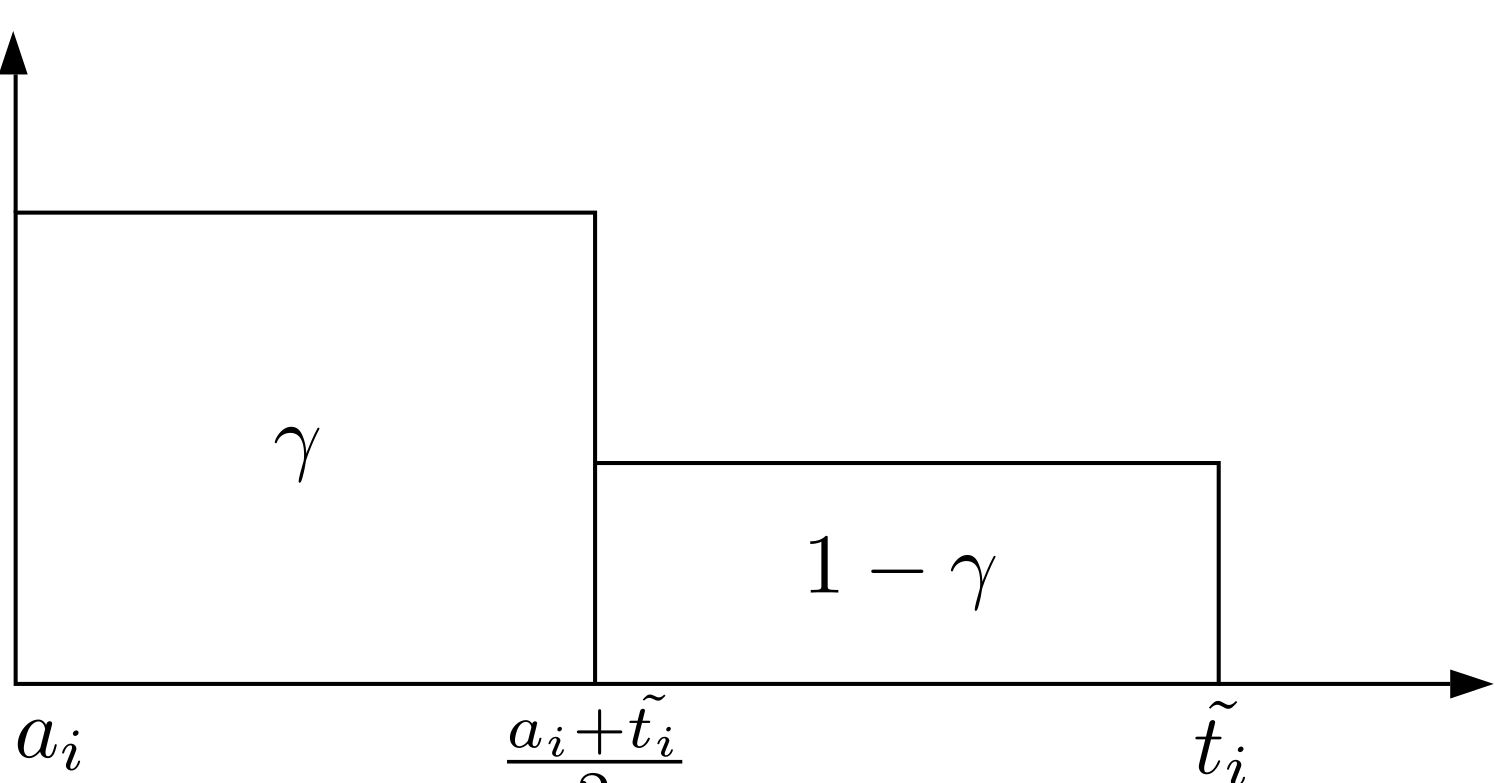
\includegraphics{fig/gendreau2006_distribution.eps}
    \caption{Distribuição do limite inferior da janela de tempo de coleta dos
             pedidos \cite{gendreau_neighborhood_2006}}
    \label{fig:gendreau2006_distribution}
\end{figure}

\noindent em que, $\mu$ simboliza a probabilidade do limite inferior da janela 
de tempo de coleta estar contido no intervalo $[\arrivalTime_\request; 
\frac{\arrivalTime_\request + \Tilde{t}_\request}{2}]$, e é definido por:
%
\begin{equation}
  \mu = \uniformDistribution{0,6}{1,0}.
\end{equation}

Já o limite superior da janela de tempo de coleta é definido por:
%
\begin{equation}
    \latestTimeWindow_\originIndex = 
      \earliestTimeWindow_\originIndex 
      + \tau(\planingHorizon - \arrivalTime_\request),
\end{equation}

\noindent em que, $\tau(\planingHorizon - \arrivalTime_\request)$ 
representa uma fração do tempo entre o instante de chegada do pedido e o fim 
do horizonte de planejamento. Assim, $\tau$ é definido por:
%
\begin{equation}
  \tau = \uniformDistribution{\tau^{\min}}{\tau^{\max}},
\end{equation}

\noindent com $\tau^{\min}$ e $\tau^{\max}$ são parâmetros determinados pelo 
usuário, cujos valores podem variar com o tempo e localização.

Uma janela de tempo é gerada da mesma forma para o local de entrega. 
Neste caso a distribuição de probabilidade para a geração do limite inferior 
da janela de tempo de entrega, como mostrado na 
Figura~\ref{fig:gendreau2006_distribution}, é definido sobre o intervalo
$[\earliestTimeWindow_\originIndex 
+ \arcTravelTime{\originIndex}{\destinationIndex}^{\min}, 
\Tilde{t} + \arcTravelTime{\originIndex}{\destinationIndex}^{\min}]$.
Já o limite superior da janela de tempo de entrega é também definido como uma
fração do intervalo de tempo entre o limite inferior da janela de tempo de
entrega e o instante final do horizonte de planejamento.

O tempo de serviço é igual a 5 minutos em cada local de serviço e um pedido é 
aceito somente quando existe no mínimo 30 minutos entre o instante de chegada 
do pedido e o último instante de coleta 
($\latestTimeWindow_\request - \requestArrivalTime \geq 30$). 
Os valores para os parâmetros $\tau$ usados para a geração das janelas de tempo
foram tomados a partir do sorteio de distribuições uniformes 
$\uniformDistribution{0,1}{0,8}$ e $\uniformDistribution{0,3}{1,0}$.

A Tabela~\ref{tab:gendreau2006_instances_characteristics} apresenta algumas
características das instâncias apresentadas por
\textcite{gendreau_neighborhood_2006}

\begin{table}[h]
\footnotesize
    \caption{Características das instâncias DPDPTW de 
             \textcite{gendreau_neighborhood_2006}}
    \label{tab:gendreau2006_instances_characteristics}
    \centering
    \begin{tabular}{lrr|lrr}
        \toprule
         ID & $\planingHorizon$ & $\numberOfRequests$ & 
         ID & $\planingHorizon$ & $\numberOfRequests$ \\
         \midrule
         req\_rapide\_1\_240\_24 & 240 &  84 & 
         req\_rapide\_3\_450\_24 & 450 & 206 \\ 
         req\_rapide\_1\_240\_33 & 240 & 144 & 
         req\_rapide\_4\_450\_24 & 450 & 217 \\
         req\_rapide\_1\_450\_24 & 240 & 169 & 
         req\_rapide\_4\_240\_24 & 240 &  90 \\ 
         req\_rapide\_2\_450\_24 & 450 & 176 &
         req\_rapide\_5\_240\_24 & 240 &  85 \\
         req\_rapide\_2\_240\_24 & 240 &  94 &
         req\_rapide\_5\_240\_33 & 240 & 153 \\
         req\_rapide\_2\_240\_33 & 240 & 112 &
         req\_rapide\_5\_450\_24 & 450 & 202 \\
         req\_rapide\_3\_240\_24 & 240 &  93 &
         req\_rapide\_5\_450\_24 & 450 & 202 \\
         req\_rapide\_3\_240\_33 & 240 & 111 &
                                 &     &     \\
         \bottomrule
  \end{tabular}
\end{table}





\section{Conjunto de instâncias DPDPTW propostas por 
         Mitrovic-Minic e Laporte (2004) e Mitrovic-
         Minic, Krishnamurti e Laporte (2004)}

Composto por dois subconjuntos de instâncias, cada um contendo 30 instâncias de 
100, 30 instâncias de 500 e 30 instâncias de 1000 pedidos.
Estes conjuntos diferem apenas em relação à distribuição e largura das 
janelas de tempo, que dependem do tempo máximo permitido para servir o pedido, 
assumindo que o pedido é coletado no primeiro instante possível, e são dadas 
por:
%
\begin{equation}
    \Gamma = \latestTimeWindow_{\destinationIndex}
              - \earliestTimeWindow_\originIndex.
    \label{eq: mitrovic_maximal_time_allowed}
\end{equation}


Os pedidos são gerados baseados em dados reais coletados em duas companhias de 
correio de médio e grande porte que operam em Vancouver, Canadá.
No primeiro conjunto a distribuição de pedidos é representada por: 
20\% pedidos com $\Gamma$ = 1 h, 30\% pedidos com $\Gamma$ = 2 h e 
50\% pedidos com $\Gamma$ = 4 h.
No segundo conjunto a distribuição é representada por: 10\% dos pedidos com 
$\Gamma$ = 1 h, 20\% dos pedidos com $\Gamma$ = 2 h, 30\% dos pedidos com 
$\Gamma$ = 4 h, 30\% dos pedidos com $\Gamma$ = 6 h 
e 10\% dos pedidos com $\Gamma$ = 8 h.

O horizonte de planejamento é de 10 h, a área de serviço é de $60 \times 60$ 
km$^2$, e a velocidade do veículo é de 60 km/h. 
Os instantes de chegada dos pedidos ocorrem dentro do horizonte de planejamento
de acordo com uma distribuição uniforme contínua e nenhum pedido é conhecido 
a priori,
%
\begin{equation}
  \arrivalTime_\request = \uniformDistribution{0}{\planingHorizon}.
\end{equation}


Um pedido $\request$ é criado através da seguinte sequência de procedimentos: 
(i) gerar o instante de chegada, 
(ii) gerar aleatoriamente as posições de coleta e entrega e 
(iii) gerar um valor para $\Gamma$.
(iv) calcular os limites das janelas de tempo como:
%
\begin{equation}
  \earliestTimeWindow_\originIndex = \arrivalTime_\request,
\end{equation}
%
\begin{equation}
  \latestTimeWindow_{\destinationIndex} = \earliestTimeWindow_\originIndex +
  \Gamma,
\end{equation}
%
\begin{equation}
  \latestTimeWindow_\originIndex = \latestTimeWindow_{\destinationIndex}
  - \arcTravelTime{i}{i+n},
\end{equation}
%
\begin{equation}
  \earliestTimeWindow_{\destinationIndex} = \earliestTimeWindow_\originIndex
  + \arcTravelTime{i}{i+n}.
\end{equation}

Rejeições de pedidos e violações de janelas de tempo não são permitidas. 
Isso é feito possível pelo fato que a quantidade de veículos 
($\vehiclesSetSize$) é considerada ilimitada. 
A frota inicial considerada é de 20, 60 e 80 veículos para as instâncias com 
100, 500 e 1000 pedidos, respectivamente. 
O ponto de início é posicionado em (20, 30) km.




